% !TEX TS-program = pdflatex
% !TEX encoding = UTF-8 Unicode

% This is a simple template for a LaTeX document using the "article" class.
% See "book", "report", "letter" for other types of document.

\documentclass[11pt,a4paper,twoside,openany]{report}

% Nicer fonts
\usepackage[T1]{fontenc}
\usepackage{lmodern}

%%% Examples of Article customizations
% These packages are optional, depending whether you want the features they provide.
% See the LaTeX Companion or other references for full information.

%%% PAGE DIMENSIONS
\usepackage[inner=2cm,outer=4cm]{geometry}

\usepackage{graphicx} % support the \includegraphics command and options
\usepackage{fixltx2e}

% \usepackage[parfill]{parskip} % Activate to begin paragraphs with an empty line rather than an indent

%%% PACKAGES
\usepackage{booktabs} % for much better looking tables
\usepackage{array} % for better arrays (eg matrices) in maths
\usepackage{paralist} % very flexible & customisable lists (eg. enumerate/itemize, etc.)
\usepackage{verbatim} % adds environment for commenting out blocks of text & for better verbatim
\usepackage{subfig} % make it possible to include more than one captioned figure/table in a single float
% These packages are all incorporated in the memoir class to one degree or another...

%%% HEADERS & FOOTERS
\usepackage{fancyhdr} % This should be set AFTER setting up the page geometry
\pagestyle{fancy} % options: empty , plain , fancy
\renewcommand{\headrulewidth}{0pt} % customise the layout...
\lhead{}\chead{}\rhead{}
\lfoot{}\cfoot{\thepage}\rfoot{}

%%% ToC (table of contents) APPEARANCE
\usepackage[nottoc,notlof,notlot]{tocbibind} % Put the bibliography in the ToC
\usepackage[titles,subfigure]{tocloft} % Alter the style of the Table of Contents
\renewcommand{\cftsecfont}{\rmfamily\mdseries\upshape}
\renewcommand{\cftsecpagefont}{\rmfamily\mdseries\upshape} % No bold!

% Hyperlinks, URLs etc.
\usepackage{hyperref}
\usepackage{url}
\hypersetup{
    colorlinks=true,
    citecolor=black,
    urlcolor=black,
    linkcolor=black,
    pagecolor=black,
    anchorcolor=black
}

% Listings
%\usepackage{chngcntr} % Renumbering done further down because the
                      % counter is only available after the document
                      % begins, for some reason.
\usepackage{listings}
\usepackage[usenames,dvipsnames]{color}

\definecolor{LightGray}{rgb}{0.9,0.9,0.9}

\lstset{basicstyle=\footnotesize\ttfamily}
\lstset{showstringspaces=false}
\lstset{numbers=none}
\lstset{keywordstyle=\color{MidnightBlue}\bfseries}
\lstset{commentstyle=\color{JungleGreen}}
\lstset{identifierstyle=\color{OliveGreen}}
\lstset{stringstyle=\color{Red}}
\lstset{backgroundcolor=\color{LightGray}}
\lstset{breaklines=true}
\lstset{captionpos=b}

\usepackage{enumitem}


\begin{document}

\pagestyle{empty}
\begin{titlepage}
                % \newgeometry{top=25mm,bottom=25mm,left=38mm,right=32mm}
                \setlength{\parindent}{0pt}
                \setlength{\parskip}{0pt}
                % \fontfamily{phv}\selectfont

                {
                                \Large
                                \raggedright
                                Imperial College London\\[17pt]
                                Department of Electrical and Electronic Engineering\\[17pt]
                                Final Year Project Report 2015\\[17pt]
 
                }

                \rule{\columnwidth}{3pt}
                \setlength{\tabcolsep}{0pt}

                \begin{tabular}{p{40mm}p{\dimexpr\columnwidth-40mm}}
                                Project Title: & \textbf{Parallelising TestU01} \\[12pt]
                                Student: & \textbf{Romanos Skiadas} \\[12pt]
                                CID: & \textbf{00693828} \\[12pt]
                                Course: & \textbf{EIE3} \\[12pt]
                                Project Supervisor: & \textbf{Dr D.B. Thomas} \\[12pt]
                                Second Marker: & \textbf{Dr T.J.W. Clarke} \\
                \end{tabular}
\end{titlepage}


\cleardoublepage

\begin{abstract}
Random Number Generators are a critical part in cryptographic algorithms as well as financial simulations, in which lack of randomness results in inaccurate results which can cause very high costs. Thus test suites to evaluate the randomness of such generators are critical.

One of the most widely used such suites is Testu01. It provides a wide variety of tests and a very well defined specification for use with software generators. However, it lacks in speed, as the tests are run in sequence, not utilising the capabilities of modern multi-core processors.

This lack of scaling becomes apparent in the larger test suites, whose run time lies in the order of hours. This project is an attempt to parallelise the three common suites of Testu01, smallCrush, Crush and BigCrush, and compare the performance of the different implementations.
\end{abstract}


\cleardoublepage
\pagestyle{plain}
\pagenumbering{roman}
\setcounter{page}{1}
\tableofcontents

\newpage
\cleardoublepage
\pagenumbering{arabic}

\include{01-introduction}
\chapter{Research}
\label{cha:res}
This chapter provides a high level introduction to the concepts required to understand the functionality of Testu01. It also provides a guide to the control flow of the parts of the suite that have been parallelised. 
Furthermore, it examines previous attempts at creating parallel versions of Testu01. It explains the shortcomings of these attempts and the novelty in this implementation of a parallel Testu01.

\section{Current state of Testu01}
Testu01 is a C library that provides collections of tests, called test suites or batteries, for testing Random Number Generators. It provides a very extensive collection of tests that can be used to ensure that Random Number Generators adhere to adequate standards of quality. The tests allow "statistical testing of uniform random number generators"\cite{testu01-homepage}.

Apart from the tests, Testu01 is distributed with example programs that use batteries to test generators, as well as reference generators that are followed by warnings against using them in critical applications. Combined with a very thorough documentation, it is a very user friendly library and can be set up and used quickly by beginners.

The documentation is a particularly strong asset of Testu01. The Short and Full Guide pdf files are generated automatically from .tex sources during the build process. These same .tex sources are also used to generate the header files for the C code. As a result, the documentation is tightly integrated with the source code. It can be used both as conventional documentation that provides guidance in using Testu01 and as a guide to understanding the control flow of the source code and extending its functionality.

Testu01 also specifies very clear interfaces for generators. Files and generators implemented in software can be used as long as they adhere to the Testu01 specifications.

Despite its usability and extensive collection of tests, Testu01 suffers from performance issues. It was not designed to take advantage of multi-core processors. A singular instance of a generator can exist at each time and it cannot be shared between tests that run concurrently. The consequence of this is that if a battery is run on an idle multi-core system, one of the cores will be constantly at maximal capacity while the rest remain idle or are used exclusively for other processes.

\begin{figure}[h]
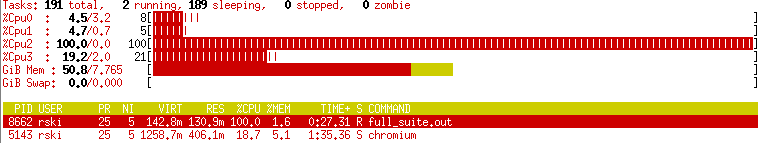
\includegraphics[scale=0.5]{top_full_suite}
\caption{Top displaying CPU usage while a test suite from Vanilla Testu01 is running\cite{full-suite}}
\label{fig:cpu_serial_tests}
\end{figure}

\section{Previous Solutions}
\subsection{Parallel Implementation of the Testu01 Statistical Test Suite}
This is one of the oldest parallel Testu01 implementations. Suciu et al. parallelised two of the test suites using OpenMP and demonstrated a relatively high increase in performance for them. Although the profiling results are promising, this solution is quite limited. The reasons for that are explained bellow.

The suites that were parallelised are \textit{Alphabit} and \textit{Rabbit}. According to the Testu01 Long Guide\cite{longguide-alphabit}, these are batteries written to test hardware generators and can be run both on files and software based generators.

Suciu et al. achieved parallelism by using threads on top of the OpenMP parallel programming API\cite{openmp}. This allowed for fine grained control over which parts of the processing where shared between threads. Sharing the generators between threads, which is the biggest hurdle in parallelising Testu01, was overcome by copying the generators at the start of every thread. 

Using this approach, the first implementation of the Rabbit and Alphabit batteries was designed and implemented, ParTestU01. Although it did provide performance gains, the first test of Rabbit was significantly slower than the rest, as it accounted for roughly half of the execution time of the battery. This prevented ParTestU01 from scaling properly, as it was always limited to the execution time of the first test.

Thus, ParTestU01E was implemented. This takes advantage of the OpenMP capabilities in order to split the first test of Rabbit into more than one processes. This provided even more performance gains.

Ultimately, the speed up increase peaked between 5 and 9 threads. Increasing the thread number beyond nine was actually detrimental to the battery performance. Running parallel Rabbit on a 32MB and a 64MB file achieved an up to six times performance increase.

It would seem that these improvements brought to the test suite are quite significant. Unfortunately, they are not, especially compared to other suites. According to the Testu01 Guide, the file based Alphabit suite running on a 1.7Ghz processor takes 2.3 minutes to test a 2\textsuperscript{30} bit file. Similarly, Rabbit requires 28 minutes to test a file of the same size. Compared to running BigCrush with a simple generator, whose runtime is above three and a half hours on a much more modern processor, these times pale in comparison.

Furthermore, neither source code or binaries for this implementation seem to be available online. The paper provides an overview of the process of parallelising Testu01, but the project apparently is unpublished for wide distribution or extremely had to discover.

Finally the authors mention that they had started working on a new and improved parallel implementation at the time that this paper was published.

\subsection{Parallel Object-Oriented Implementation of the Testu01 Statistical Test Suites}
This is the paper that follows the previous one by Suciu et al. The same research group parallelised a different part of Testu01 using an Object Oriented approach. This is a very promising implementation with impressive performance gains compared to the original Testu01.

Once again, only part of Testu01 was parallelised. This was the Multinomial distribution test, as according to the authors this "is by far the most time consuming statistical test from Testu01". This solution is quite complex and was decided due to limitations of C, which could be overcome by features of OOP.

Generators for this solution were implemented using interfaces. In contrast with the original generator definitions, this allows for concurrent generators.The fact that generator data is now encapsulated along with functions for copying and initialising generators, allowed for concurrent generators.

Since C does not support object oriented programming, this solution was implemented in C\#. Similarly, OpenMP that was previously used had to be replaced with the Task Parallel Library (TPL).

Using these as a basis, the Multinomial Distribution Test was parallelised and performance metrics were gathered. The speedup is quite close but consistently higher than the one of the OpenMP implementation of this test.

The greatest advantage of this implementation is that it can be used to parallelise the rest of the tests of Testu01. Unfortunately, no paper on the progress of porting Testu01 to this TPL solution could be found.

\section{The Case for yet Another Solution}
\subsection{Problems with the current solutions}
Perhaps the biggest limitation of the previous solutions is their non-completeness. Testu01 is a very extensive library and provides a great number of batteries, tests and generators. These solutions improve a small fraction of them. There are still test suites that have runtimes of hours and could benefit greatly from multi-core scaling.

There is also still demand for a parallelised Testu01 that requires small changes in projects that already using Testu01. An implementation that uses the current  Testu01 specifications will have lower use barriers for projects that have conformed to them.

Furthermore, converting the entirety of Testu01 using these solutions is a time consuming and difficult challenge. The OpenMP solution turned out to not be usable outside of the Alphabit and Rabbit batteries, so it is not possible to use it as a guide for parallelising the rest of Testu01. Similarly, moving to TPL and C\# requires a considerable amount of effort. This project provides a solution that could be used to quickly parallelise any test suite and generator.

BigCrush is a test suite whose total run time exceeds three hours on a system with an Intel i5-3570k processor, with four cores clocked at 3.4Ghz. This suite calls 106 test functions, each one of which might run more than one test. Converting all these tests to a TPL based parallel suite and ensuring they still produce correct results is a task that might not be completed in the foreseeable future. This project will provide a parallel BigCrush that can be used with very minimal changes in existing programs that use Testu01 to test generators. The Crush and to a lesser extend smallCrush battery also benefit from it.

\chapter{Implementation}
\label{cha:imp}
There was a number of considerations while designing and building this solution. These ranged from time limitations to minimising the amount of chances in the original Testu01 library and producing a less complex solution. 

This chapter explains these limitations and the process of making choices in the design of the final implementation in order to best balance the solution between these limitations.

\section{Design Choices}
\subsection{Threads versus Processes}
\label{sec:processes}
The usual approach in parallelisation is to spawn threads, each of which handles a discrete part of the processing. This approach is favoured in larger projects, because it allows handling the complexity of multithreading internally, without the use of process wrappers.

The biggest advantage of threads is that they share address space. Results can be passed to the thread handler via conventional means, such as arrays. Since each test already puts its results in a specific array cell, this approach would seem natural.

Usually, thread programming is bug-prone because of the need for locking. Data corruption, deadlocks and loss of performance due to waiting for locked resources are common\cite{ers-artofunix}. Fixing these would increase overall time required to complete the project.

A multi-threaded Testu01 would not suffer from these problems. The result data of each test is already placed completely independently in an array, so locking would not be required.

However, there is a number of problems with using threads, the greatest of which is that the complexity of the changes in Testu01 would be quite high. 

The creators of Testu01 have in some cases built in it functionality that eases the decoupling of the separate tests in threads. In some others, their code is too tightly integrated together that a multi-threaded approach would require major restructuring. 

The generators are not shareable between threads. There is only one generator that the tests use in sequence. If it were to be used by threads, each thread would not get sequential increments along the generator state, effectively getting random sequences instead of deterministic ones and the test results would be skewed.

Thus the biggest challenge would be to ensure that every thread uses a separate generator. An array of generators could be used, but this would require building a function that using a single generator instance creates an array of them. This would increase complexity and potentially introduce unforeseen consequences. Restructuring the test suites so that they use the generator array would be required. Finally, the way that the result printing aggregators are called and behave would have to change. All these involve restructuring that would both require large amount of time and might introduce unforeseen consequences that could cause erroneous results.

The greatest advantage of multiple processes is that the generator separation is done automatically. A new generator for the test is created by the slave process in the exact same way that the generators are currently created.

The test suites are already designed so that only a specific test can be run when they are called. Adding the functionality needed to select a single test is trivial. Thus using processes only requires small changes in Testu01. This makes porting any future Testu01 improvements to the parallel implementation comparatively easier.

Furthermore, the process wrapper code can be written in a language other than C. Since it is not a time crucial part of the code, it can be written a higher level language such as Python, improving maintainability and extensibility.

Of course, processes have disadvantages of their own. The biggest one is the fact that the generator is set up separately for each process. This is explored further in the limitations section.

Extracting the test results from the processes will also have to be handled by the process master. Ideally they would be aggregated programmatically. Testu01 already provides this functionality and threads would be able to use it. Processes will not, so it will have to be duplicated by the process master.

Overall processes seem the better choice. Implementing them requires less time and debugging will be easier, both of which are very important under the time limitations for the project.

\subsection{Process Master Implementation Language}


\section{Building Testu01}
\subsection{Vanilla Testu01}
The project was entirely developed and tested on Arch Linux. As such, Arch specific tools were used to automate the build and install process, the most important of which is makepkg.

Testu01 can be built using the conventional ./configure make make install process. This is useful for Linux distributions for which packages with precompiled binaries do not exist. 

This is not the case for Arch Linux as a script that automates the process is provided in the Arch Linux User Repository. This way Testu01 is also handled by the package manager. The process for building packages from the AUR is explained thoroughly in the Arch Wiki\cite{archwiki-aur} and only the important parts for building Testu01 will be repeated here.

After acquiring the Testu01 PKGBUILD from the AUR\cite{testu01-aur}, it can be installed with the following commands
\begin{verbatim}
makepkg -s
sudo pacman -U testu01-1.2.3-3-$(uname -m).pkg.tar.xz
\end{verbatim}

\subsection{Modified Testu01}
Building the customised version of Testu01 only requires small changes in the PKGBUILD file to point to the correct github repository.


\section{Running the test suites}

\chapter{Results and the Future}
\label{cha:results}
In this chapter, the results are analysed with regards to performance and correctness. Furthermore the limitations of this solution are discussed as well as possible improvements for the future.

\section{Assessing Correctness}

\section{Testu01 Compatibility}

\section{Limitations and Future Work}
\subsection{Generator setup time}
Currently, the biggest limitation of this solution is the fact that a test generator is initialised every time a test is run. Since the tests run in separate processes, a new generator is set up for each one.
For trivial generators, this cost might be insignificant, but for generators that are simulations of hardware, it can overshadow the performance gains of parallelisation. The following equations can help illustrate this point:

Linear test suite completion time: N * AverageTestTime + GenSetupTime
Parallel test suite completion time: N * (AverageTestTime + GenSetupTime) / NumbOfCores
Solving for GenSetupTime:

If this equation holds, then the performance of the parallel suite will be at worst the same as the serial one.
The number of cores of modern desktops and laptops ranges between two and eight. Using these numbers, estimates for the maximum efficient parallel GenSetupTime can be acquired. Since systems with more cores than eight were used in the actual measurements, estimations are included for those too.
Number of cores
2 4 6 8
smallCrush
Crush
BigCrush

\subsection{Lack of flexibility}

\subsection{Windows support}
The original test suites could be compiled for Windows. The Testu01 homepage provides precompiled Windows binaries which can be used to run the tests.

However, despite this project being theoretically still portable and working on Windows, it has not been tested for compatibility. This is due to lack of time and lack of knowledge and experience with working on Cygwin on Windows.

\subsection{File Generators}
Currently the three Crush suites allow for use of files as random number generators. This functionality has not been tested at all and was not taken under consideration when building the parallel Testu01. As a result, the best approximation that can be given for using the parallel suites with a file generator is simply undefined behaviour and should not be used at all.

However, given the nature of files, it would quite probably be possible to extend the parallelism for these generators as well without major restructuring of the code base.

\chapter{Quick Start Guide}
\section{Installation}
This is a guide on how to install and run the parallel Testu01 suite.

First clone the git repository from github\cite{github-repo}.
\begin{verbatim}
  git clone $URL
\end{verbatim}

For Arch Linux users the following step can be skipped. There is a PKGBUILD inside the build directory that can be used it install Testu01.
Refer to the Arch Wiki instructions on installing from the AUR.

Install the modified Testu01 (refer to your distributions manual and the Testu01 documentation for proper configuration):
\begin{verbatim}
  ./configure
  make
  sudo make install 
\end{verbatim}

\section{Running the tests suites}
Enter the \texttt{parallel} folder. Run make to compile the test slave executable.


Use the following command to run the parallel test suite:
\begin{verbatim}
  python proocess_master.py
\end{verbatim}

\section{Selecting the battery}
The battery can be selected by editing the \texttt{testSuite} variable in the file \texttt{process\_master}.


\begin{thebibliography}{99}

\bibitem{Testu01}
  Testu01 Homepage\\
  \url{https://www.iro.umontreal.ca/~simardr/testu01/tu01.html}\\
  Last fetched 2015-06-22.
 
\end{thebibliography}

\chapter{Appendix}

\section{Code Repositories}

\section{smallCrush Results}
\subsection{Parallel smallCrush}
\subsection{Serial smallCrush}


\end{document}
